
\subsection{Resultados de rendimiento}
\label{sec:performance-results}

\subsubsection{Tiempo de generación de claves}

\begin{table}[H]
\centering
\caption{Tiempo de generación de claves.}
\label{tab:keygen-time}
\small
\begin{tabular}{lrrrrrr}
\toprule
\textbf{Protocolo} &
\textbf{Media} &
\textbf{Mediana} &
\textbf{Desv.} &
\textbf{P95} &
\textbf{P99} &
\textbf{Máx.} \\
&
\multicolumn{6}{c}{\textbf{ms}} \\
\midrule

ECDSA       & \todoresult{} & \todoresult{} & \todoresult{} & \todoresult{} & \todoresult{} & \todoresult{} \\
LWE         & \todoresult{} & \todoresult{} & \todoresult{} & \todoresult{} & \todoresult{} & \todoresult{} \\
Binary-LWE  & \todoresult{} & \todoresult{} & \todoresult{} & \todoresult{} & \todoresult{} & \todoresult{} \\
Ring-LWE    & \todoresult{} & \todoresult{} & \todoresult{} & \todoresult{} & \todoresult{} & \todoresult{} \\
LWR         & \todoresult{} & \todoresult{} & \todoresult{} & \todoresult{} & \todoresult{} & \todoresult{} \\
LWE propio  & \todoresult{} & \todoresult{} & \todoresult{} & \todoresult{} & \todoresult{} & \todoresult{} \\

\bottomrule
\end{tabular}
\end{table}


% ============================================================
\subsubsection{Tiempo de autenticación}

\begin{table}[H]
\centering
\caption{Tiempo promedio por etapa del proceso de autenticación.}
\label{tab:authentication-time}
\small
\begin{tabularx}{\textwidth}{lCCCCC}
\toprule
\textbf{Protocolo} &
\textbf{Challenge} &
\textbf{Response} &
\textbf{Verify} &
\textbf{Total} &
\textbf{Throughput} \\
&
\textbf{ms} &
\textbf{ms} &
\textbf{ms} &
\textbf{ms} &
\textbf{auth/s} \\
\midrule

ECDSA      & \todoresult{} & \todoresult{} & \todoresult{} & \todoresult{} & \todoresult{} \\
LWE        & \todoresult{} & \todoresult{} & \todoresult{} & \todoresult{} & \todoresult{} \\
Binary-LWE & \todoresult{} & \todoresult{} & \todoresult{} & \todoresult{} & \todoresult{} \\
Ring-LWE   & \todoresult{} & \todoresult{} & \todoresult{} & \todoresult{} & \todoresult{} \\
LWR        & \todoresult{} & \todoresult{} & \todoresult{} & \todoresult{} & \todoresult{} \\
LWE propio & \todoresult{} & \todoresult{} & \todoresult{} & \todoresult{} & \todoresult{} \\

\bottomrule
\end{tabularx}
\end{table}


% ============================================================
\subsubsection{Distribución de los tiempos}

La Figura~\ref{fig:auth-time-comparison} presenta el tiempo medio requerido para
completar una autenticación.

\begin{figure}[H]
\centering

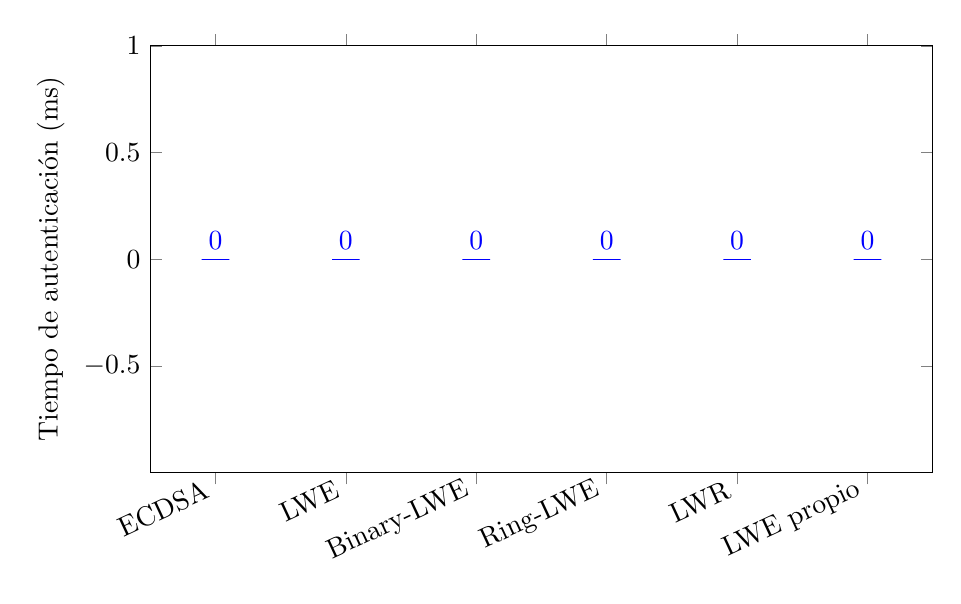
\begin{tikzpicture}
\begin{axis}[
    ybar,
    width=0.95\textwidth,
    height=7cm,
    ylabel={Tiempo de autenticación (ms)},
    symbolic x coords={ECDSA,LWE,Binary-LWE,Ring-LWE,LWR,LWE propio},
    xtick=data,
    x tick label style={rotate=25,anchor=east},
    nodes near coords,
    ymin=0,
    enlarge x limits=0.1
]
\addplot coordinates {
    (ECDSA,0)
    (LWE,0)
    (Binary-LWE,0)
    (Ring-LWE,0)
    (LWR,0)
    (LWE propio,0)
};
\end{axis}
\end{tikzpicture}

\caption{Comparación del tiempo medio de autenticación.
Reemplazar los valores cero por los resultados experimentales.}
\label{fig:auth-time-comparison}
\end{figure}

Los resultados muestran que \todoresult{describir los resultados observados sin
interpretarlos todavía}. La diferencia entre \todoresult{protocolos relevantes} fue
de \todoresult{valor}, mientras que \todoresult{resultado adicional}.


% ============================================================
\subsection{Resultados de consumo de memoria}
\label{sec:memory-results}

\begin{table}[H]
\centering
\caption{Consumo de memoria durante las operaciones criptográficas.}
\label{tab:memory-results}
\small
\begin{tabularx}{\textwidth}{lCCCC}
\toprule
\textbf{Protocolo} &
\textbf{RAM media} &
\textbf{RAM pico} &
\textbf{Estado temporal} &
\textbf{Estado persistente} \\
&
\textbf{KB} &
\textbf{KB} &
\textbf{KB} &
\textbf{bytes/usuario} \\
\midrule

ECDSA      & \todoresult{} & \todoresult{} & \todoresult{} & \todoresult{} \\
LWE        & \todoresult{} & \todoresult{} & \todoresult{} & \todoresult{} \\
Binary-LWE & \todoresult{} & \todoresult{} & \todoresult{} & \todoresult{} \\
Ring-LWE   & \todoresult{} & \todoresult{} & \todoresult{} & \todoresult{} \\
LWR        & \todoresult{} & \todoresult{} & \todoresult{} & \todoresult{} \\
LWE propio & \todoresult{} & \todoresult{} & \todoresult{} & \todoresult{} \\

\bottomrule
\end{tabularx}
\end{table}


% ============================================================
\subsection{Tamaño de claves y estructuras criptográficas}
\label{sec:key-size-results}

\begin{table}[H]
\centering
\caption{Tamaño serializado de los principales objetos criptográficos.}
\label{tab:key-sizes}
\small
\begin{tabularx}{\textwidth}{lCCCC}
\toprule
\textbf{Protocolo} &
\textbf{Clave pública} &
\textbf{Clave privada} &
\textbf{Parámetros públicos} &
\textbf{Total registro} \\
&
\textbf{bytes} &
\textbf{bytes} &
\textbf{bytes} &
\textbf{bytes} \\
\midrule

ECDSA      & \todoresult{} & \todoresult{} & \todoresult{} & \todoresult{} \\
LWE        & \todoresult{} & \todoresult{} & \todoresult{} & \todoresult{} \\
Binary-LWE & \todoresult{} & \todoresult{} & \todoresult{} & \todoresult{} \\
Ring-LWE   & \todoresult{} & \todoresult{} & \todoresult{} & \todoresult{} \\
LWR        & \todoresult{} & \todoresult{} & \todoresult{} & \todoresult{} \\
LWE propio & \todoresult{} & \todoresult{} & \todoresult{} & \todoresult{} \\

\bottomrule
\end{tabularx}
\end{table}


% ============================================================
\subsection{Resultados de comunicación}
\label{sec:communication-results}

\begin{table}[H]
\centering
\caption{Datos transmitidos durante una autenticación.}
\label{tab:communication}
\small
\begin{tabularx}{\textwidth}{lCCCCC}
\toprule
\textbf{Protocolo} &
\textbf{Challenge} &
\textbf{Response} &
\textbf{Metadata} &
\textbf{Total} &
\textbf{Mensajes} \\
&
\textbf{bytes} &
\textbf{bytes} &
\textbf{bytes} &
\textbf{bytes} &
\\
\midrule

ECDSA      & \todoresult{} & \todoresult{} & \todoresult{} & \todoresult{} & \todoresult{} \\
LWE        & \todoresult{} & \todoresult{} & \todoresult{} & \todoresult{} & \todoresult{} \\
Binary-LWE & \todoresult{} & \todoresult{} & \todoresult{} & \todoresult{} & \todoresult{} \\
Ring-LWE   & \todoresult{} & \todoresult{} & \todoresult{} & \todoresult{} & \todoresult{} \\
LWR        & \todoresult{} & \todoresult{} & \todoresult{} & \todoresult{} & \todoresult{} \\
LWE propio & \todoresult{} & \todoresult{} & \todoresult{} & \todoresult{} & \todoresult{} \\

\bottomrule
\end{tabularx}
\end{table}


% ============================================================
\subsection{Escalabilidad de almacenamiento}
\label{sec:storage-scalability}

A partir del almacenamiento requerido por usuario se estima el espacio necesario para
diferentes tamaños del sistema.

Si $S_u$ representa el almacenamiento persistente requerido por usuario, entonces:

\begin{equation}
    S(N) = N S_u.
\end{equation}

\begin{table}[H]
\centering
\caption{Estimación de almacenamiento según el número de usuarios.}
\label{tab:storage-scalability}
\small
\begin{tabularx}{\textwidth}{lCCCC}
\toprule
\textbf{Protocolo} &
\textbf{1 usuario} &
\textbf{1.000 usuarios} &
\textbf{100.000 usuarios} &
\textbf{1.000.000 usuarios} \\
\midrule

ECDSA      & \todoresult{} & \todoresult{} & \todoresult{} & \todoresult{} \\
LWE        & \todoresult{} & \todoresult{} & \todoresult{} & \todoresult{} \\
Binary-LWE & \todoresult{} & \todoresult{} & \todoresult{} & \todoresult{} \\
Ring-LWE   & \todoresult{} & \todoresult{} & \todoresult{} & \todoresult{} \\
LWR        & \todoresult{} & \todoresult{} & \todoresult{} & \todoresult{} \\
LWE propio & \todoresult{} & \todoresult{} & \todoresult{} & \todoresult{} \\

\bottomrule
\end{tabularx}
\end{table}


% ============================================================
\subsection{Evaluación de seguridad}
\label{sec:security-evaluation}

La seguridad de las alternativas basadas en retículos no se determina únicamente por
el nombre de la familia criptográfica. Depende de los parámetros concretos
seleccionados para cada implementación.

Por este motivo, para cada candidato se documentan los parámetros y la estimación de
seguridad correspondiente.

\begin{table}[H]
\centering
\caption{Nivel de seguridad estimado para las configuraciones evaluadas.}
\label{tab:security-levels}
\small
\begin{tabularx}{\textwidth}{lYCCC}
\toprule
\textbf{Protocolo} &
\textbf{Problema base} &
\textbf{Seguridad clásica} &
\textbf{Seguridad cuántica} &
\textbf{Método de estimación} \\
\midrule

ECDSA &
ECDLP &
\todoresult{} &
\todoresult{} &
\todoresult{} \\

LWE &
LWE &
\todoresult{} &
\todoresult{} &
\todoresult{} \\

Binary-LWE &
LWE con secreto binario &
\todoresult{} &
\todoresult{} &
\todoresult{} \\

Ring-LWE &
Ring-LWE &
\todoresult{} &
\todoresult{} &
\todoresult{} \\

LWR &
LWR &
\todoresult{} &
\todoresult{} &
\todoresult{} \\

LWE propio &
\todoresult{} &
\todoresult{} &
\todoresult{} &
\todoresult{} \\

\bottomrule
\end{tabularx}
\end{table}

Cuando se utilicen estimadores de seguridad, deberán registrarse también la versión de
la herramienta, sus parámetros de entrada y los modelos de costo utilizados.


% ============================================================